\documentclass[10pt,a4paper]{article}
\usepackage[utf8]{inputenc}
\usepackage{amsmath}
\usepackage{amsfonts}
\usepackage{amssymb}
\usepackage{tikz}
\usetikzlibrary{datavisualization}
\usetikzlibrary{datavisualization.formats.functions}
\usepackage[left=25mm,right=25mm]{geometry}
\usepackage{pgfplots}
\usepgfplotslibrary{external} 
\tikzexternalize
\usepackage{float} 
\usepackage{multicol}
\usepackage{hyperref}


\graphicspath{ {./figures/} }

\begin{document}
\begin{multicols}{2}
\newenvironment{indentPar}[1]%
 {\begin{list}{}%
         {\setlength{\leftmargin}{#1}}%
         \item[]%
 }
 {\end{list}}

\begin{flushleft}
\begin{LARGE}EE 535 Lab 4: Quantum Efficiency
\end{LARGE}	
\\Jonathan Hess
\\\href{https://github.com/Jetsama/EE535/tree/main/Lab4}{https://github.com/Jetsama/EE535/tree/main/Lab4}
\end{flushleft}


\section*{Abstract}
Quantum efficiency is the efficiency of a material to convert incoming photons into output, such as electricity. An unknown quantum efficiency of a Perovskite, calcium titanium oxide(CaTiO3),solar cell sample and a unknown crystalline silicon solar cell sample were tested and measured. They were then compared against a reference silicon photo diode with a known quantum efficiency.
	





\section*{Introduction}






\section*{Definitions}
Quantum Efficiency (QE) is the efficiency of a material to convert incoming photons into output, such as electricity.\\


Internal Quantum Efficiency (IQE) is the efficiency with which a device  converts absorbed photons into electron-hole pairs within the material.\\
External Quantum Efficiency (EQE) measures the efficiency of a device to convert absorbed photons into electrical current that is collected at the device's terminals.\\
Incident photons ($N_o$) the photons that hit the material.

Transmission (T) is the amount of light and electromagnetic radiation that passes through a media.\\
Reflection (R) is the amount of light and electromagnetic radiation that changes direction. \\
Absorbance (A) is the measure of how much light is absorbed by a substance at a particular wavelength.\\



\section*{Experimental}
During this lab measurements of quantum efficiency was done with 
The material tested would be centered where the output was the strongest. Then the lock on amplifier Model SR830 DSP Lock-In Amplifier was used to measure the exact voltages across the photo diode.


\begin{figure}[H]\centering\label{meascurrent}

\includegraphics[scale=0.25]{measuringcurrent}
\caption{Diagram for current and voltage measurements of photo diode}
\end{figure}
These measurements would be done on both the known quantum efficiency silicon and the unknown samples and compared.\\
To create the light a bulb was used alongside light filtering devices. The Jobin Yvon monochromator took this input light and filtered the output. Alongside other glass filters there is an assumed mono frequency light beam going to the photodiode. This allowed for measurement seeps at specific frequencies.



\section*{Theory}

In figure \ref{meascurrent} the current going through the resistor is can be shown with equation \ref{eq:photocurrent}.\\

\begin{equation}\label{eq:photocurrent}
I = -I_{ph} + I_s (e^{\frac{V}{V_t}}-1)
\end{equation}
Where I is the current across the resistor, V is the voltage of the diode, $V_t$ is the thermal voltage, and $I_{ph}$ is the photo current created by the diode.\\
There are two conditions to consider.\\
The first is as the resistor reaches an infinite resistance the current equation derives to equation . This is because the current going through the resistor (I) will be 0. This means $I_{ph}$ must equation the diode current.\\
The second is when the resistor is shorted the current equation derives to equation \ref{eq:photocurrentshort}. This is because the current of resistor is equal to the photo current.

\begin{equation}\label{eq:photocurrentshort}
I_{sc} = -I_{ph}
\end{equation}
\begin{equation}\label{eq:photocurrentinfinteR}
I_{ph} = I_s (e^{\frac{V}{V_t}}-1)
\end{equation}

The voltage of the diode can be found with the infinite resistance equation \ref{eq:photocurrentinfinteR}.

\begin{equation}\label{eq:photovoltageinfinteR}
V = ln(\frac{I_{ph}}{I_s+1}) V_t
\end{equation}

For quantum efficiency equation \ref{eq:QE} can be used  in combination with for measuring.\\
\begin{equation}\label{eq:QE}
QE = \frac{\textrm{number of collected EHP}}{\textrm{number of incidental photons}}
\end{equation}

\begin{equation}\label{eq:N0}
N(x) = N_0 e^{-\alpha x}
\end{equation}
Where $N$ is absorbed photons, $N_0$ is the number of incident photons, and alpha is the absorption coefficient of the material.

\begin{equation}\label{eq:Gx}
G(x) =   - \frac{d N(x)}{ d x}
\end{equation}
To calculated the generation of EHPs the derivative can be taken to get the rate of absorbed EHP then multiplied by negative one to get generation. This yeilds equation \ref{eq:Gx}.
\begin{equation}\label{eq:Bx}
b(x) =  e^{-\alpha x}
\end{equation}

\begin{equation}\label{eq:NC}
N_c = \frac{L_p}{\alpha QL_p +1} \alpha N_0
\end{equation}

Internal quantum efficiency is the measurement of the internal electron hole pairs (EHP) of the device. This can be found with the following equation.

\begin{equation}\label{eq:IQE}
IQE = \frac{\alpha L_p}{QL_p +1}
\end{equation}

Using equation \ref{eq:IQE} to solve for $L_p$ using graphing methods.

\begin{equation}\label{eq:IQE}
\frac{1}{IQE} = 1+ \frac{1}{\alpha L_p}
\end{equation}
Where the x values are $\frac{1}{\alpha}$ and y values are $\frac{1}{IQE}$ yields a slope of $\frac{1}{L_p}$.

\begin{equation}\label{eq:EQE}
EQE = \frac{IQE}{1-R}
\end{equation}
Where R is reflection of the material.  

Diffusion Length
\begin{equation}\label{eq:difLen}
L = \sqrt{D\tau}
\end{equation}


Photo current density
\begin{equation}\label{eq:difLen}
J_{\text{ph}} = \int_{0}^{\lambda_0} \varepsilon N Q E(x) \,d\lambda
\end{equation}
Where $\varepsilon$ represents the elementary charge, N represents the number of photons, Q represents the charge of an electron or electron-hole pair, E(x) represents the external quantum efficiency (EQE) as a function of wavelength(x), and $\lambda$ represents the wavelength of light.


\begin{equation}\label{eq:difLen}
\frac{D}{\mu} = \frac{kt}{q}
\end{equation}




\section*{Results}
The reference silicon photo diode has a reported quantum efficiency given by figure \ref{refQE}. What needs to be calculated is the voltages 
expected with these quantum effienciencies. Then a comparison against the measured voltages can show error in the currents of the sample.
\begin{figure}[H]\centering\label{refQE}
\includegraphics[scale=0.5]{ReferenceQE}
\caption{Graph for wavelength vs quantum efficiency for the reference silicon photo diode}
\end{figure}
This given refernce can then be compared against the measured values of the reference given in figure \ref{refQEMeas}.
\begin{figure}[H]\centering\label{refQEMeas}
%\includegraphics[scale=0.5]{ReferenceQEMeas}
\caption{Graph for wavelength vs quantum efficiency for the reference silicon photo diode}
\end{figure}


\section*{Appendix}
For information on the pure data or computational scripts there is a repository for this and other labs. \\
https://github.com/Jetsama/EE535\\
\begin{thebibliography}{9}
\bibitem{book}
 Solid State Electronic Devices (2006, Prentice Hall), Ben Streetman, Sanjay Banerjee
 
\bibitem{LockIn}
\href{https://www.thinksrs.com/downloads/pdfs/manuals/SR830m.pdf}{MODEL SR830 DSP Lock-In Amplifier Manual}
\bibitem{Green}
Green, M.A. and Keevers, M. "Optical properties of intrinsic silicon at 300 K ", Progress in Photovoltaics, p.189-92, vol.3, no.3; (1995)

\bibitem{Lasers}
An Entry Level Guide to Understanding Lasers (2008), Chapter 9.2.4, Jeff Hecht, 3rd ed. 

\bibitem{paper}
R Swanepoel 1983 J. Phys. E: Sci. Instrum. 16 1214

\bibitem{optical}
Optical Processes in Semiconductors, Jacques I. Pankove

\bibitem{carry}
Cary 100/300/4000/5000/6000i/7000 Spectrophotometers User's Guide

\bibitem{tauc}
How To Correctly Determine the Band Gap Energy of Modified Semiconductor Photocatalysts Based on UV–Vis Spectra, Patrycja Makuła, Michał Pacia, and Wojciech Macyk\\https://pubs.acs.org/doi/10.1021/acs.jpclett.8b02892
\bibitem{semi}
Silicon Photo Multipliers Detectors Operating in Geiger Regime: an Unlimited Device for Future Applications,Giancarlo Barbarino, Riccardo de Asmundis, Gianfranca De Rosa, Carlos Maximiliano Mollo, Stefano Russo and Daniele Vivolo


\bibitem{peaks} \href{https://erdogant.github.io/findpeaks/pages/html/Examples.html#find-peaks-in-low-sampled-dataset}{text}


\bibitem{marq} E Marquez et al 1992 J. Phys. D: Appl. Phys. 25 535
\bibitem{siK}Handbook of Optical Constants of Solids, Edward D. Palik. Academic Press, Boston, 1985 
\end{thebibliography}


\end{multicols}
\end{document}
